\documentclass[a4paper, 11pt, spanish]{article}
\usepackage[spanish, mexico]{babel}
\usepackage[utf8]{inputenc}
\usepackage{graphicx}
\usepackage{epstopdf}
\usepackage{csquotes}
\usepackage{booktabs}
\usepackage{helvet}
\usepackage{mathptmx}
\usepackage{geometry}
\usepackage{upquote}
\usepackage{spreadtab}
\usepackage{import}
\usepackage{sectsty}
%%%%%%%%%%%%%%%%%%%%%%%%%%%%%%%%%%%%%%%%%%%%%%%%%%%%%%%%
\usepackage[dvipsnames]{xcolor}
\definecolor{azulOscuro}{rgb}{0.0, 0.28, 0.67}
\definecolor{verdeCopado}{rgb}{0.13, 0.55, 0.13}
%%%%%%%%%%%%%%%%%%%%%%%%%%%%%%%%%%%%%%%%%%%%%%%%%%%%%%%%
\usepackage[acronym, toc, style=list]{glossaries}
%\usepackage[xindy, acronym, toc, style=list]{glossaries}
\makeglossaries
\loadglsentries[main]{glosario.tex}
%%%%%%%%%%%%%%%%%%%%%%%%%%%%%%%%%%%%%%%%%%%%%%%%%%%%%%%%
\usepackage{appendix}
\allsectionsfont{\normalfont\sffamily\bfseries}
\renewcommand{\appendixname}{Apéndice}
\renewcommand{\appendixtocname}{Apéndice}
\renewcommand{\appendixpagename}{\normalfont\bfseries Apéndice}
\usepackage{etoolbox} % we load it for the workaround
% workaround
\makeatletter
\appto{\appendices}{\def\Hy@chapapp{Appendix}}
\makeatother
%%%%%%%%%%%%%%%%%%%%%%%%%%%%%%%%%%%%%%%%%%%%%%%%%%%%%%%
\usepackage{listings}
\lstset{
	language=HTML,
	numbers=left,
	stepnumber=1,    
	firstnumber=1,
	numberfirstline=true,
	postbreak=\raisebox{0ex}[0ex][0ex]{\ensuremath{\color{red}\hookrightarrow\space}},
	xleftmargin=1.5cm,
	xrightmargin=1.5cm,
	frame=shadowbox,
	rulesepcolor=\color{black},
	captionpos=b,
	abovecaptionskip=12pt,
	framextopmargin=0.2cm,
	framexbottommargin=0.2cm,
	framexleftmargin=0.8cm,
	framexrightmargin=0.8cm,
	numbersep=0.3cm,
	breaklines=true,columns=fullflexible,
	basicstyle=\small\normalfont,
	extendedchars=true,
	literate=
	{á}{{\'a}}1 {é}{{\'e}}1 {í}{{\'i}}1 {ó}{{\'o}}1 {ú}{{\'u}}1
	{Á}{{\'A}}1 {É}{{\'E}}1 {Í}{{\'I}}1 {Ó}{{\'O}}1 {Ú}{{\'U}}1
}

\renewcommand{\lstlistingname}{Fragmento}

%\lstset{basicstyle=\footnotesize\ttfamily}
%%%%%%%%%%%%%%%%%%%%%%%%%%%%%%%%%%%%%%%%%%%%%%%%%%%%%%%
\usepackage{tikz}
\usepackage{setspace}
\usepackage{hyperref} % Es para la url o el indice
\hypersetup{
	colorlinks=true,
	linkcolor=black,
	citecolor=verdeCopado,
	filecolor=PineGreen,
	urlcolor=azulOscuro,
	linktoc=all,
	pdftitle={Informe de proyecto 1}
}
\usepackage{cite}
\usepackage{apacite}
\bibliographystyle{apacite}
\AtBeginDocument{
	\renewcommand{\BBOP}{[}
	\renewcommand{\BBCP}{]}
}

\usepackage{datetime}% http://ctan.org/pkg/datetime
\newdateformat{mifecha}{La Plata, \monthname[\THEMONTH] de \THEYEAR}
\makeatletter
\renewcommand{\monthnamespanish}[1][\month]{%
	\@orgargctr=#1\relax
	\ifcase\@orgargctr
	\PackageError{datetime}{Invalid Month number \the\@orgargctr}{%
		Month numbers should go from 1 to 12}%
	\or Enero%
	\or Febrero%
	\or Marzo%
	\or Abril%
	\or Mayo%
	\or Junio%
	\or Julio%
	\or Agosto%
	\or Septiembre%
	\or Octubre%
	\or Noviembre%
	\or Diciembre%
	\else \PackageError{datetime}{Invalid Month number \the\@orgargctr}{%
		Month numbers should go from 1 to 12}%
	\fi}

% Caratula:
	% En Primer hoja. Especificar título del proyecto, autores y fecha.

\renewcommand{\maketitle}{%
	\begin{titlepage}
		\singlespacing
		\begin{center}
			\begin{minipage}[t][7.6cm]{10.5cm}
				\begin{center}
					\centering
					{
\includegraphics[width=1\textwidth]{imagenes/logos.pdf}\par}
					\vspace{2cm}
					{\Large\textbf{Informe final}\par}\vfill
					{\LARGE\textbf{Cartel lumínico configurable por WiFi}\par}\vfill
					\vspace{10mm}
					{\Large Taller de proyecto 1 (E0306)\par}
					\vspace{4cm}
					{\large Grupo 07}\\
					\vspace{5mm}
					{\large
						\begin{tabular}{rl}
							García & Agustín \\
							Levy& Santiago \\
							Romero~Dapozo& Ramiro \\
							Ternouski& Sebastian~Nahuel\\
						\end{tabular}
					}
				\end{center}
			\end{minipage}
			\vfill
			{\large \par \mifecha\today \par}
		\end{center}
	\end{titlepage}
	\if@twoside
	\thispagestyle{empty}
	\cleardoublepage
	\else
	\addtocounter{page}{1}
	\fi
}
\usepackage{wrapfig}

\newcommand{\code}[1]{\mbox{#1}}

\begin{document}
	\renewcommand\refname{Bibliografías} % Para cambiar el nombre referencias a Bibliografias.
	\hypersetup{pageanchor=false}
	\maketitle
	\tableofcontents % indice de contenidos
	\addtocontents{toc}{\protect\thispagestyle{empty}}
	\clearpage
	\hypersetup{pageanchor=true}

	\setcounter{page}{1}
	% Para estilizar código
\section{Introducción}
% TODO: insertar chamu sobre sistemas similares disponibles, etc.
En el ámbito universitario resulta necesario mantener informadas a las personas sobre una amplia variedad de hechos, noticias y acontecimientos que sucedieron o sucederán, desde la ubicación de un aula hasta la notificación de la cancelación de una clase. Muchas veces estas notificaciones son sobre cuestiones muy efímeras, lo que requiere rapidez para empezar a transmitirlas y facilidad para tener el alcance necesario.

En las facultades de la Universidad Nacional de La Plata se consumen muchos recursos para cumplir este fin, a través de afiches, pancartas, panfletos, etc. los cuales, pese a ser de barata fabricación, no tienen una vida útil muy extensa. Además todas estas formas de comunicación se basan en el uso de papel, que tras ser utilizado debe desecharse debido a la imposibilidad de reutilizarlo, generando una cantidad de residuos significativa. Si se tiene en cuenta que también generan una polución visual considerable, por la gran cantidad de estos distribuidos en todos los lugares transitables, resulta prudente considerar una nueva forma de comunicación.

% TODO: Mencionar sobre otros carteles comercialmente disponibles
Surge así la idea de desarrollar de un cartel electrónico reutilizable, capaz de ser configurado remotamente por las autoridades competentes, con el fin de proveer una forma de comunicación masiva más limpia, clara y menos dañina para el medio ambiente.

En este informe se describe todas las fases del desarrollo de un proyecto para la asignatura Taller de Proyecto 1. El proyecto consiste en el diseño y desarrollo de un sistema de cartel luminoso cuyo contenido es configurable de forma remota. El cartel tiene conectividad WiFi, con lo que es capaz de formar parte de una red IP.

El proyecto utilizó un proceso de desarrollo de cascada, como se muestra en la figura \ref{fig:waterfall}.

\begin{figure}[!ht]
	\centering
	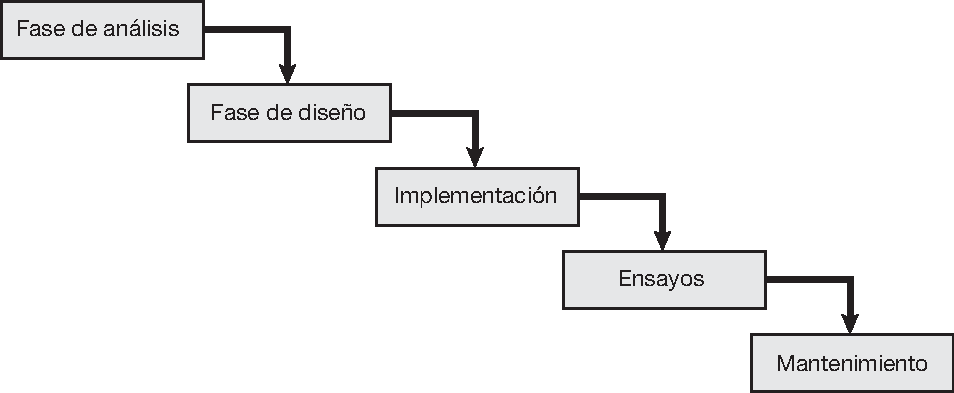
\includegraphics[width=0.8\linewidth]{imagenes/waterfall.pdf}
	\caption{Modelo en cascada de desarrollo.}
	\label{fig:waterfall}
\end{figure}

A lo largo de este informe se documentarán las fases de desarrollo previamente mencionadas.

En la sección \ref{part:analisis} se habla sobre los requerimientos y especificaciones del sistema, detallando que funcionalidades debe tener y a cuáles restricciones está sujeto.

Luego, en la sección \ref{part:diseno}, se mencionan las componentes que constituyen el sistema, se explicitan modelos que describen el comportamiento del sistema, la interfaz de usuario y la arquitectura del software. También se muestran los esquemáticos que especifican la conexión de los componentes.

En la sección de implementación se documenta como se fue dando el proceso de desarrollo de software y la implementación física del hardware.

En la sección de ensayos se documenta los resultados de las pruebas que se realizaron sobre el sistema en funcionamiento.

Por último, se anexa como apéndice una guía instructiva que explica los pasos necesarios para poner en marcha el sistema.

\section{Objetivos del proyecto}
El objetivo primario de este proyecto es el diseño implementación de un cartel luminoso que pueda ser configurado remotamente por un usuario. No se tiene como objetivo realizar un producto diseñado de manera que sea económicamente viable producirlo en masa, sino más bien el desarrollo de un prototipo a modo de prueba de concepto.

El objetivo puede ser divido en los siguientes subobjetivos:
\begin{itemize}
	\item Diseño general de la solución.
	\item Diseño e implementación del hardware que controla el cartel.
	\item Diseño e implementación del software mediante el cual se establece el contenido del cartel de forma remota.
	\item Diseño e implementación del protocolo de comunicación por el cual interactuarán las componentes.
\end{itemize}

En la parte \ref{part:analisis} se explicitará las funcionalidades que debe tener el sistema y la interfaz de usuario que expone.


% ==============================================================
\clearpage
\part{Análisis de requerimientos}\label{part:analisis}
\section{Requerimientos}
\subsection{Funcionales}
\begin{itemize}
	\item La aplicación de PC deberá ser capaz de poder iniciar una conexión segura con el sistema utilizando la misma para enviar los mensajes que el cliente desee.
	\item La aplicación podrá enviar peticiones de forma de obtener el mensaje actual del cartel o incluso establecer uno nuevo. Por otra parte, también podrá pedir los datos de la red a la que el sistema estará conectado o cambiarlos.
	\item La aplicación deberá ser capaz de modificar parámetros de animación tales como frecuencia de parpadeo y velocidad de desplazamiento lateral o estaticidad.
	\item La aplicación permitirá al usuario, ingresar por teclado el mensaje que desea mostrar mediante los caracteres que se establecen en el estándar de codificación de caracteres ISO/IEC 8859-1 (ver \cite{CodifChar}).
	\item El cartel deberá poder procesar sólo mensajes a través del protocolo diseñado específicamente para este proyecto (ver sección \ref{sec:protocolo})
	\item El cartel deberá mostrar los mensajes que desee el usuario.
	\item El cartel deberá poder almacenar y modificar sus credenciales de red de forma de poder conectarse al WiFi que el cliente desee.
	\item El cartel deberá mantener los datos de configuración y del mensaje que muestra, aún cuando el mismo haya sido desconectado de la red inalámbrica o de la red eléctrica.
\end{itemize}

\subsection{No funcionales}
\begin{itemize}
	\item El tiempo de respuesta del cartel no debe exceder los cinco segundos.
	\item El sistema entero no debe consumir mas de 30 Watts bajo operación normal.
	\item El sistema deberá ser capaz de aceptar sólo conexiones por TLS \cite{TLS} de forma que las conexiones y el intercambio de paquetes sea cifrado y seguro.
\end{itemize}
% TODO: Hacer diagramas de caso de uso
\subsection{Interacción con el usuario}
\section{Especificaciones físicas}



% ==============================================================
\clearpage
\part{Diseño}\label{part:diseno}
\section{Hardware}\label{sec:hw}
\subsection{Diagrama en bloques general}
El sistema se compone de módulos funcionales que interactúan entre sí, estos son: el \emph{maestro}, el cual recibe los datos recibidos y los \emph{esclavos} que actualizan una matriz, en la figura \ref{fig:diagrama-bloques-general} se puede observar el diagrama en bloques de todo el sistema.

\begin{figure}[!ht]
	\centering
	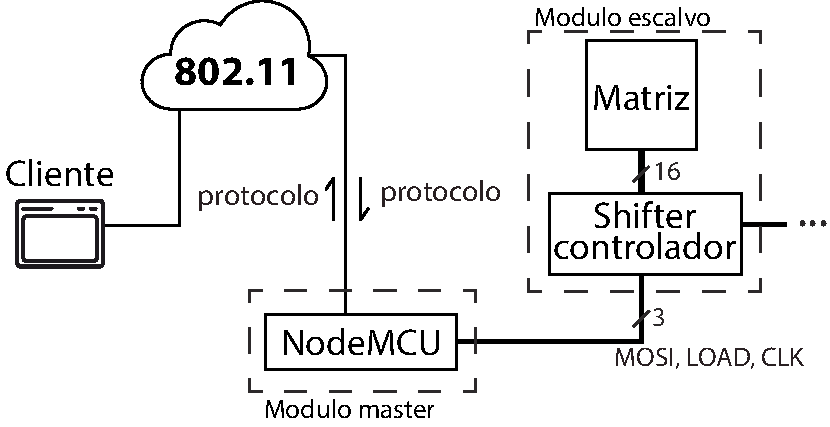
\includegraphics[width=\linewidth]{imagenes/hw/diagrama-bloques-general.pdf}
	\caption{Esquema general entre todos los componentes del sistema.}
	\label{fig:diagrama-bloques-general}
\end{figure}

\subsection{Fuente de alimentación}
El sistema recibe una fuente alimentación de forma externa, la cual es de 5V para abastecer los componentes internos. Para ello, de decidió incorporar un Jack (de 5.5mm x 2.1mm) a modo de interfaz.

\subsection{Módulo maestro}
Como se mencionó anteriormente, este modulo se encarga de procesar los datos enviados desde el cliente y controlar los demás módulos.

Su componente principal es el microcontrolador NodeMCU, que integra un AI-Thinker ESP-12E (figura \ref{fig:foto-esp12e}), el cual contiene un SoC (\emph{System on Chip}) ESP8266EX (figura \ref{fig:esp8266ex}) de la empresa Espressif. El módulo NodeMCU es hardware libre, sin embargo, el ESP12E y el ESP8266EX no lo son.\cite{NodeMCU}

\begin{figure}[ht!]
	\begin{center}
		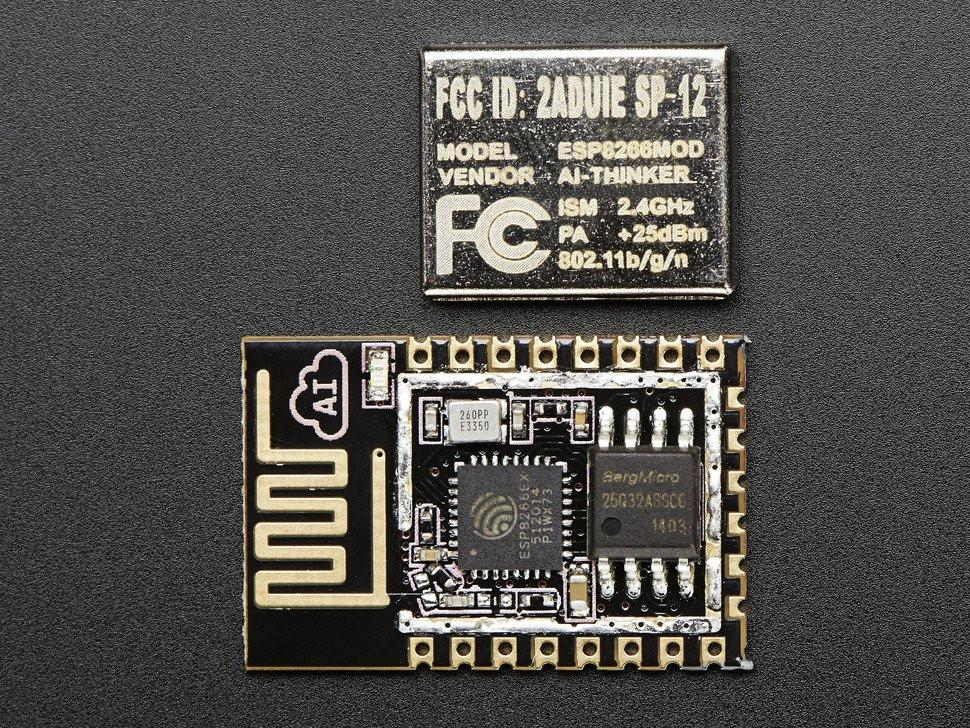
\includegraphics[width=8cm]{imagenes/esp12e-foto.jpg}
		\caption{Foto del módulo ESP12E sin su cubrimiento.}
		\label{fig:foto-esp12e}
	\end{center}
\end{figure}

\begin{figure}[ht!]
	\begin{center}
		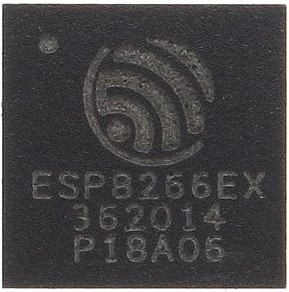
\includegraphics[width=3cm]{imagenes/esp8266ex.jpg}
		\caption{Foto del integrado ESP8266EX.}
		\label{fig:esp8266ex}
	\end{center}
\end{figure}

\begin{figure}[ht!]
	\begin{center}
		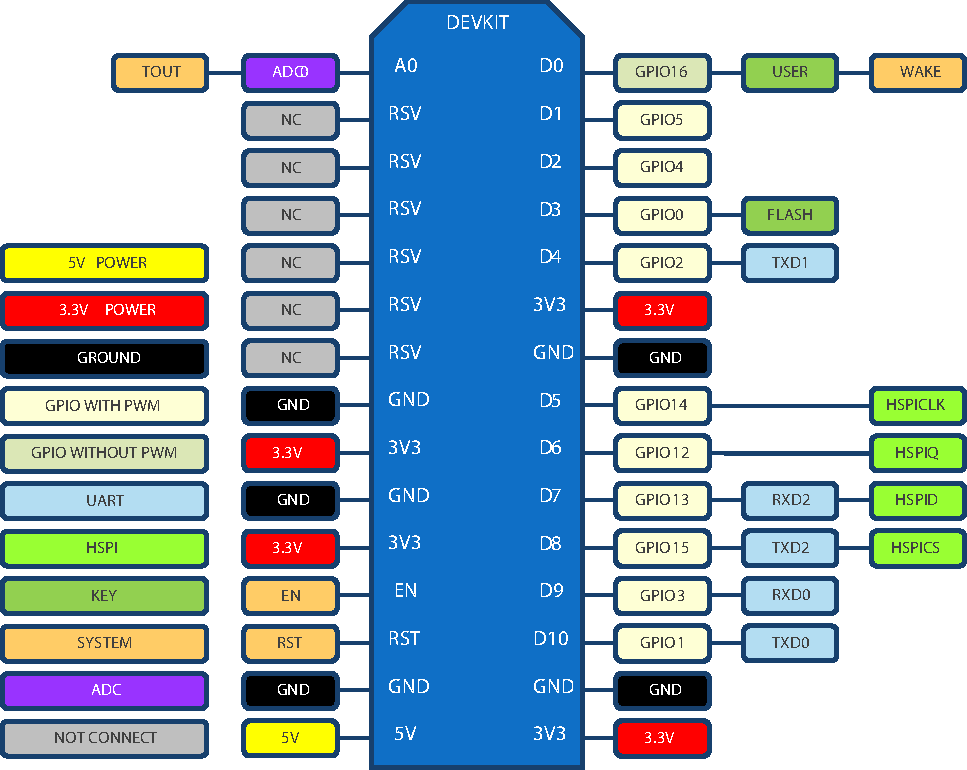
\includegraphics[width=0.95\textwidth]{imagenes/nodemcu-pinout.pdf}
		\caption{Asignación de pines del NodeMCU.}
		\label{fig:nodemcu-pinout}
	\end{center}
\end{figure}

Es importante tener en cuenta que el sistema no integra en su hardware directamente ni el ESP12E ni el ESP8266EX, sino que integra el NodeMCU, cuya asignación de pines se puede ver en la figura \ref{fig:nodemcu-pinout}.

El chip ESP8266EX combina un microcontrolador Tensillica Xtensa L106, un RISC de 32 bits corriendo a 80 Mhz, con funcionalidad WiFi. \cite{ESP8266Datasheet} El chip tiene memoria ROM con firmware no removible, y puede correr programas almacenados en flash externa. Para poder usar todas sus funcionalidades, se debe programar sobre firmware privativo desarrollado por Espressif, esto implica que el programa de usuario corre en simultáneo con el firmware y el uso de la memoria de trabajo está sujeto a la versión del firmware. Según el datasheet, el usuario puede esperar tener disponible 50 KiB de SRAM.

Como se mencionó anteriormente, se necesita de flash externa para correr programas. El módulo ESP-12S se encarga de proveer al ESP8266EX 4 MiB de memoria flash.

\subsection{Módulo esclavo}
Un modulo esclavo posee un driver MAX7219, que es el componente principal junto con una interfaz que permite conectarse a otro módulo esclavo o en su defecto al master.

\subsubsection{MAX7219}
El MAX7219 es un controlador compacto, de entrada y salida en serie de cátodo común que conectan microprocesadores a LEDs numéricos de siete segmentos de hasta ocho dígitos, pantallas de gráfico de barras o 64 LED individuales. Se incluyen en el chip, un decodificador BCD, circuitos de multiplexación, controladores de segmentos y dígitos, y una RAM estática de 8x8 que almacena cada número. Solo se necesita una resistencia externa para configurar la corriente de segmento para todos los LEDs.

El MAX7219 es compatible con los protocolos SPI, QSPI y Microwire, y tiene controladores de segmento de velocidad limitada para reducir el EMI.

Los dígitos individuales se pueden actualizar sin reescribir toda la pantalla. El MAX7219 también permite al usuario seleccionar el código de decodificación o no decodificación para cada dígito.

Su alimentación V\texttt{+} debe estar entre 4 y 5.5 Volts para su correcto funcionamiento. En cambio los voltaje de las entradas lógicas tienen una restricción de que un valor alto como mínimo debe ser 3.5V y un valor bajo como máximo 0.8V.

Las características principales que posee el chip integrado se enumeran a continuación:
\begin{itemize}
	\item Interfaz serie de 10 MHz.
	\item Control de segmento LED individual.
	\item Selección de dígitos Decode / No-Decode.
	\item Apagado de baja potencia de 150 microA (datos retenidos).
	\item Control de brillo digital y analógico.
	\item Pantalla borrada al encenderse.
	\item Unidad de visualización LED de cátodo común.
	\item SPI, QSPI, interfaz serie Microwire paquetes DIP y SO de 24 pines.
\end{itemize}

La disposición de los pines del MAX7219 se puede observar en la figura \ref{fig:MAX-pines} y la descripción de cada uno en la tabla \ref{table:MAX-pines}.

Es necesario prestar atención en el conexionado con respecto a los pines de tierra (GND) ya que ambos deben estar conectados para el driver pueda funcionar correctamente, ambas estan al lado izquierdo de la figura \ref{fig:MAX-pines} (Pin 4 y 9).

Por otro lado, el MAX7219 tiene un pin denominado DOUT (pin 24) se utiliza para encadenar varios MAX7219 y de esta forma pasar la información al que esta directamente conectado, éste pin nunca tiene alta impedancia.\\

\begin{figure}[ht!]
	\centering
	\begin{center}
	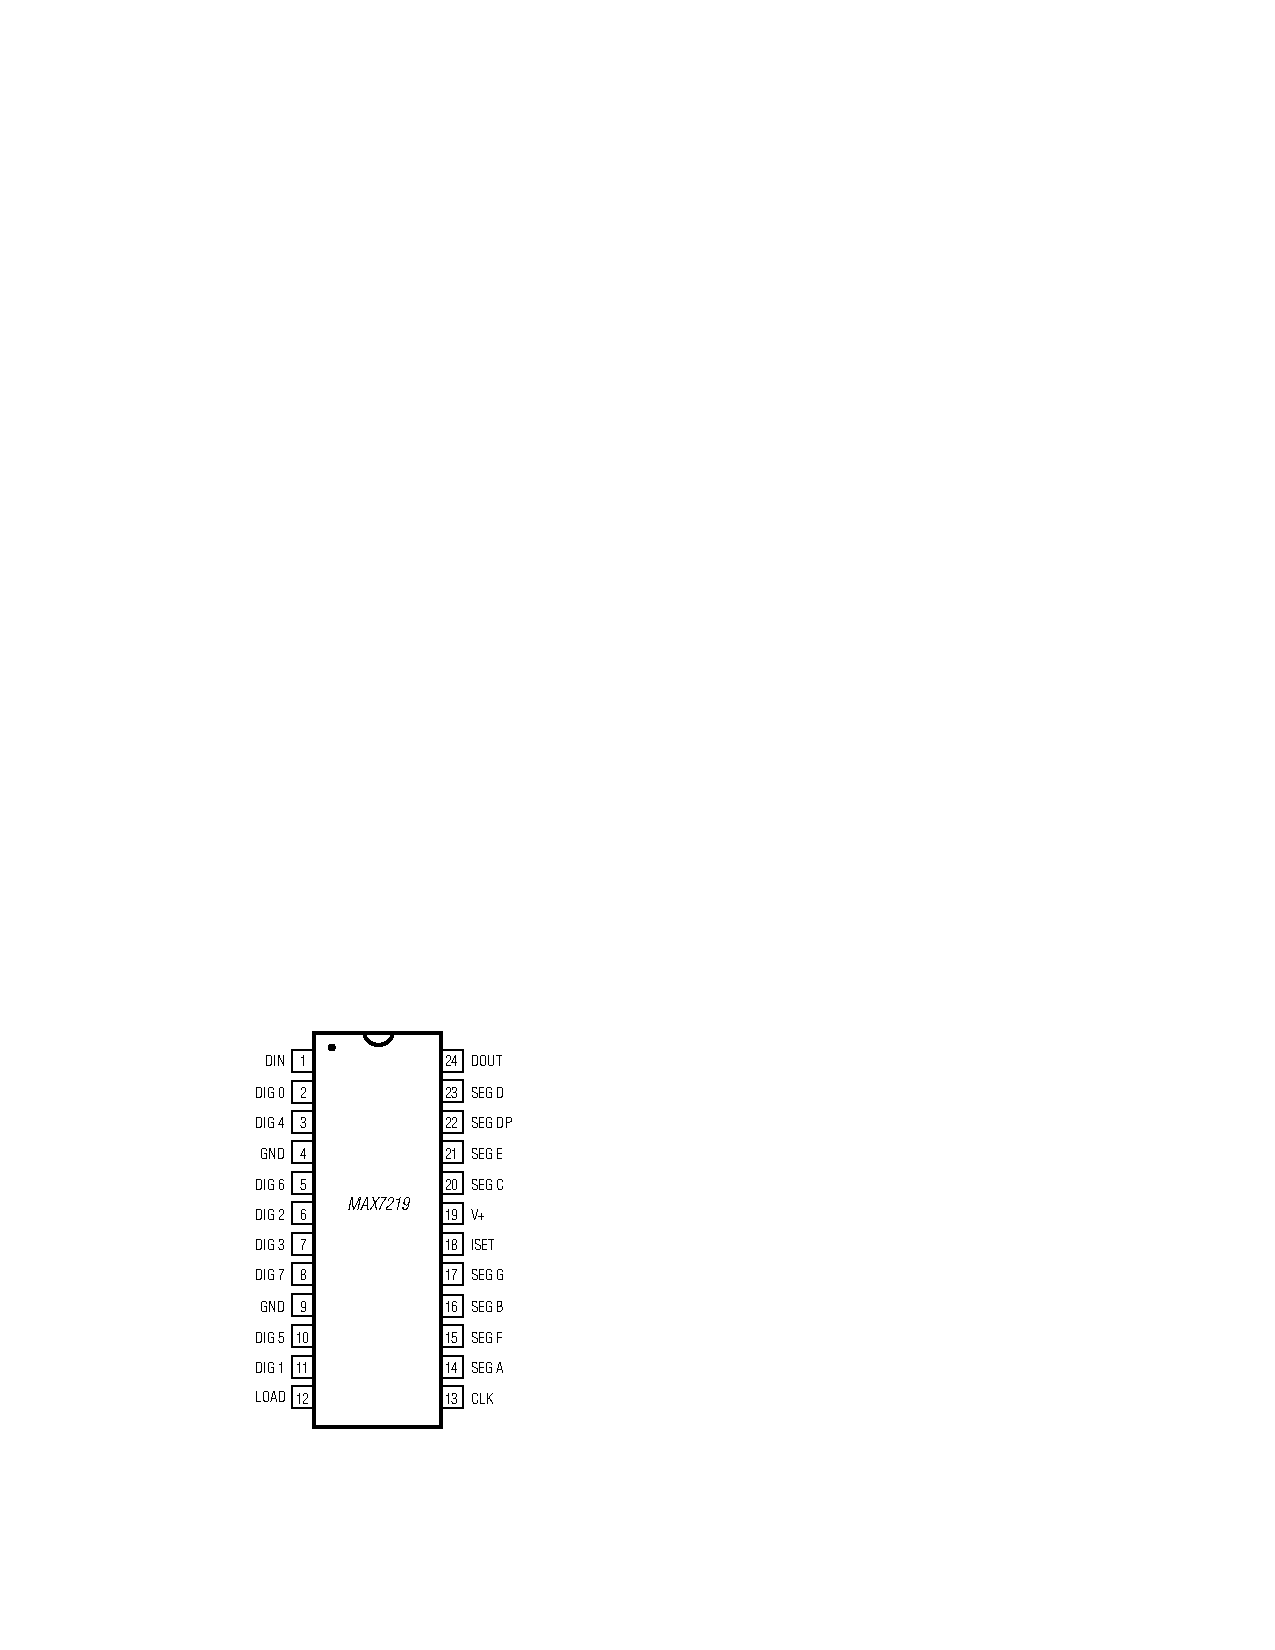
\includegraphics[scale=1.2]{imagenes/hw/max.pdf}
	 \caption{Configuración de pines del chip MAX7219.}
	  \label{fig:MAX-pines}
	\end{center}
\end{figure}

\begin{table}[ht]
\centering
\caption{Descripción de los pines del MAX7219}
\label{table:MAX-pines}
\begin{tabular}{C{10mm} C{14mm} L{108mm}}
\hline
Pin               & Nombre          & Función    \\ \hline
1                 & DIN             & Pin de datos seriales. Los datos son cargados en el registro de 16 bits en cada flanco ascendente del clock. \\
2, 3, 5–8, 10, 11 & DIG 0 - DIG 7    & Líneas de transmisión de ocho dígitos que absorben corriente del cátodo común de la pantalla. El MAX7219 deja en V+ cuando esta apagado. Los dígitos están en alta impedancia cunado se apaga.\\
4, 9              & GND             & Tierra.\\
12                & LOAD            & Pin de control. Los últimos 16 bits del Serial Data son cargados en el flanco ascendente. \\
13                & CLK             & Pin de clock serial. En cada flanco ascendente, los datos sin shifteados dentro de un registro interno. En cada flanco descendente los datos salen de DOUT. En el MAX7221, la entrada CLK está activa solo mientras LOAD está baja. \\
14–17, 20-23      & SEG A–SEG G, DP & Las unidades de siete segmentos y el punto decimal impulsan la fuente de corriente a la pantalla. Cuando un controlador de segmento está apagado, se conecta a GND.\\
18                & ISET            & Conectar a  $V_{DD}$ a través de una resistencia ($R_{SET}$) para configurar la corriente que pueda entregar a los dígitos y segmentos. \\
19                & V+              & Fuente positiva de corriente, conectar a 5 V. \\
24                & DOUT            & Salida de datos en serie. Los datos en DIN son válidos en DOUT 16.5 ciclos de reloj más tarde. \\ \hline
\end{tabular}
\end{table}

\begin{figure}[ht!]
\centering
\begin{center}
	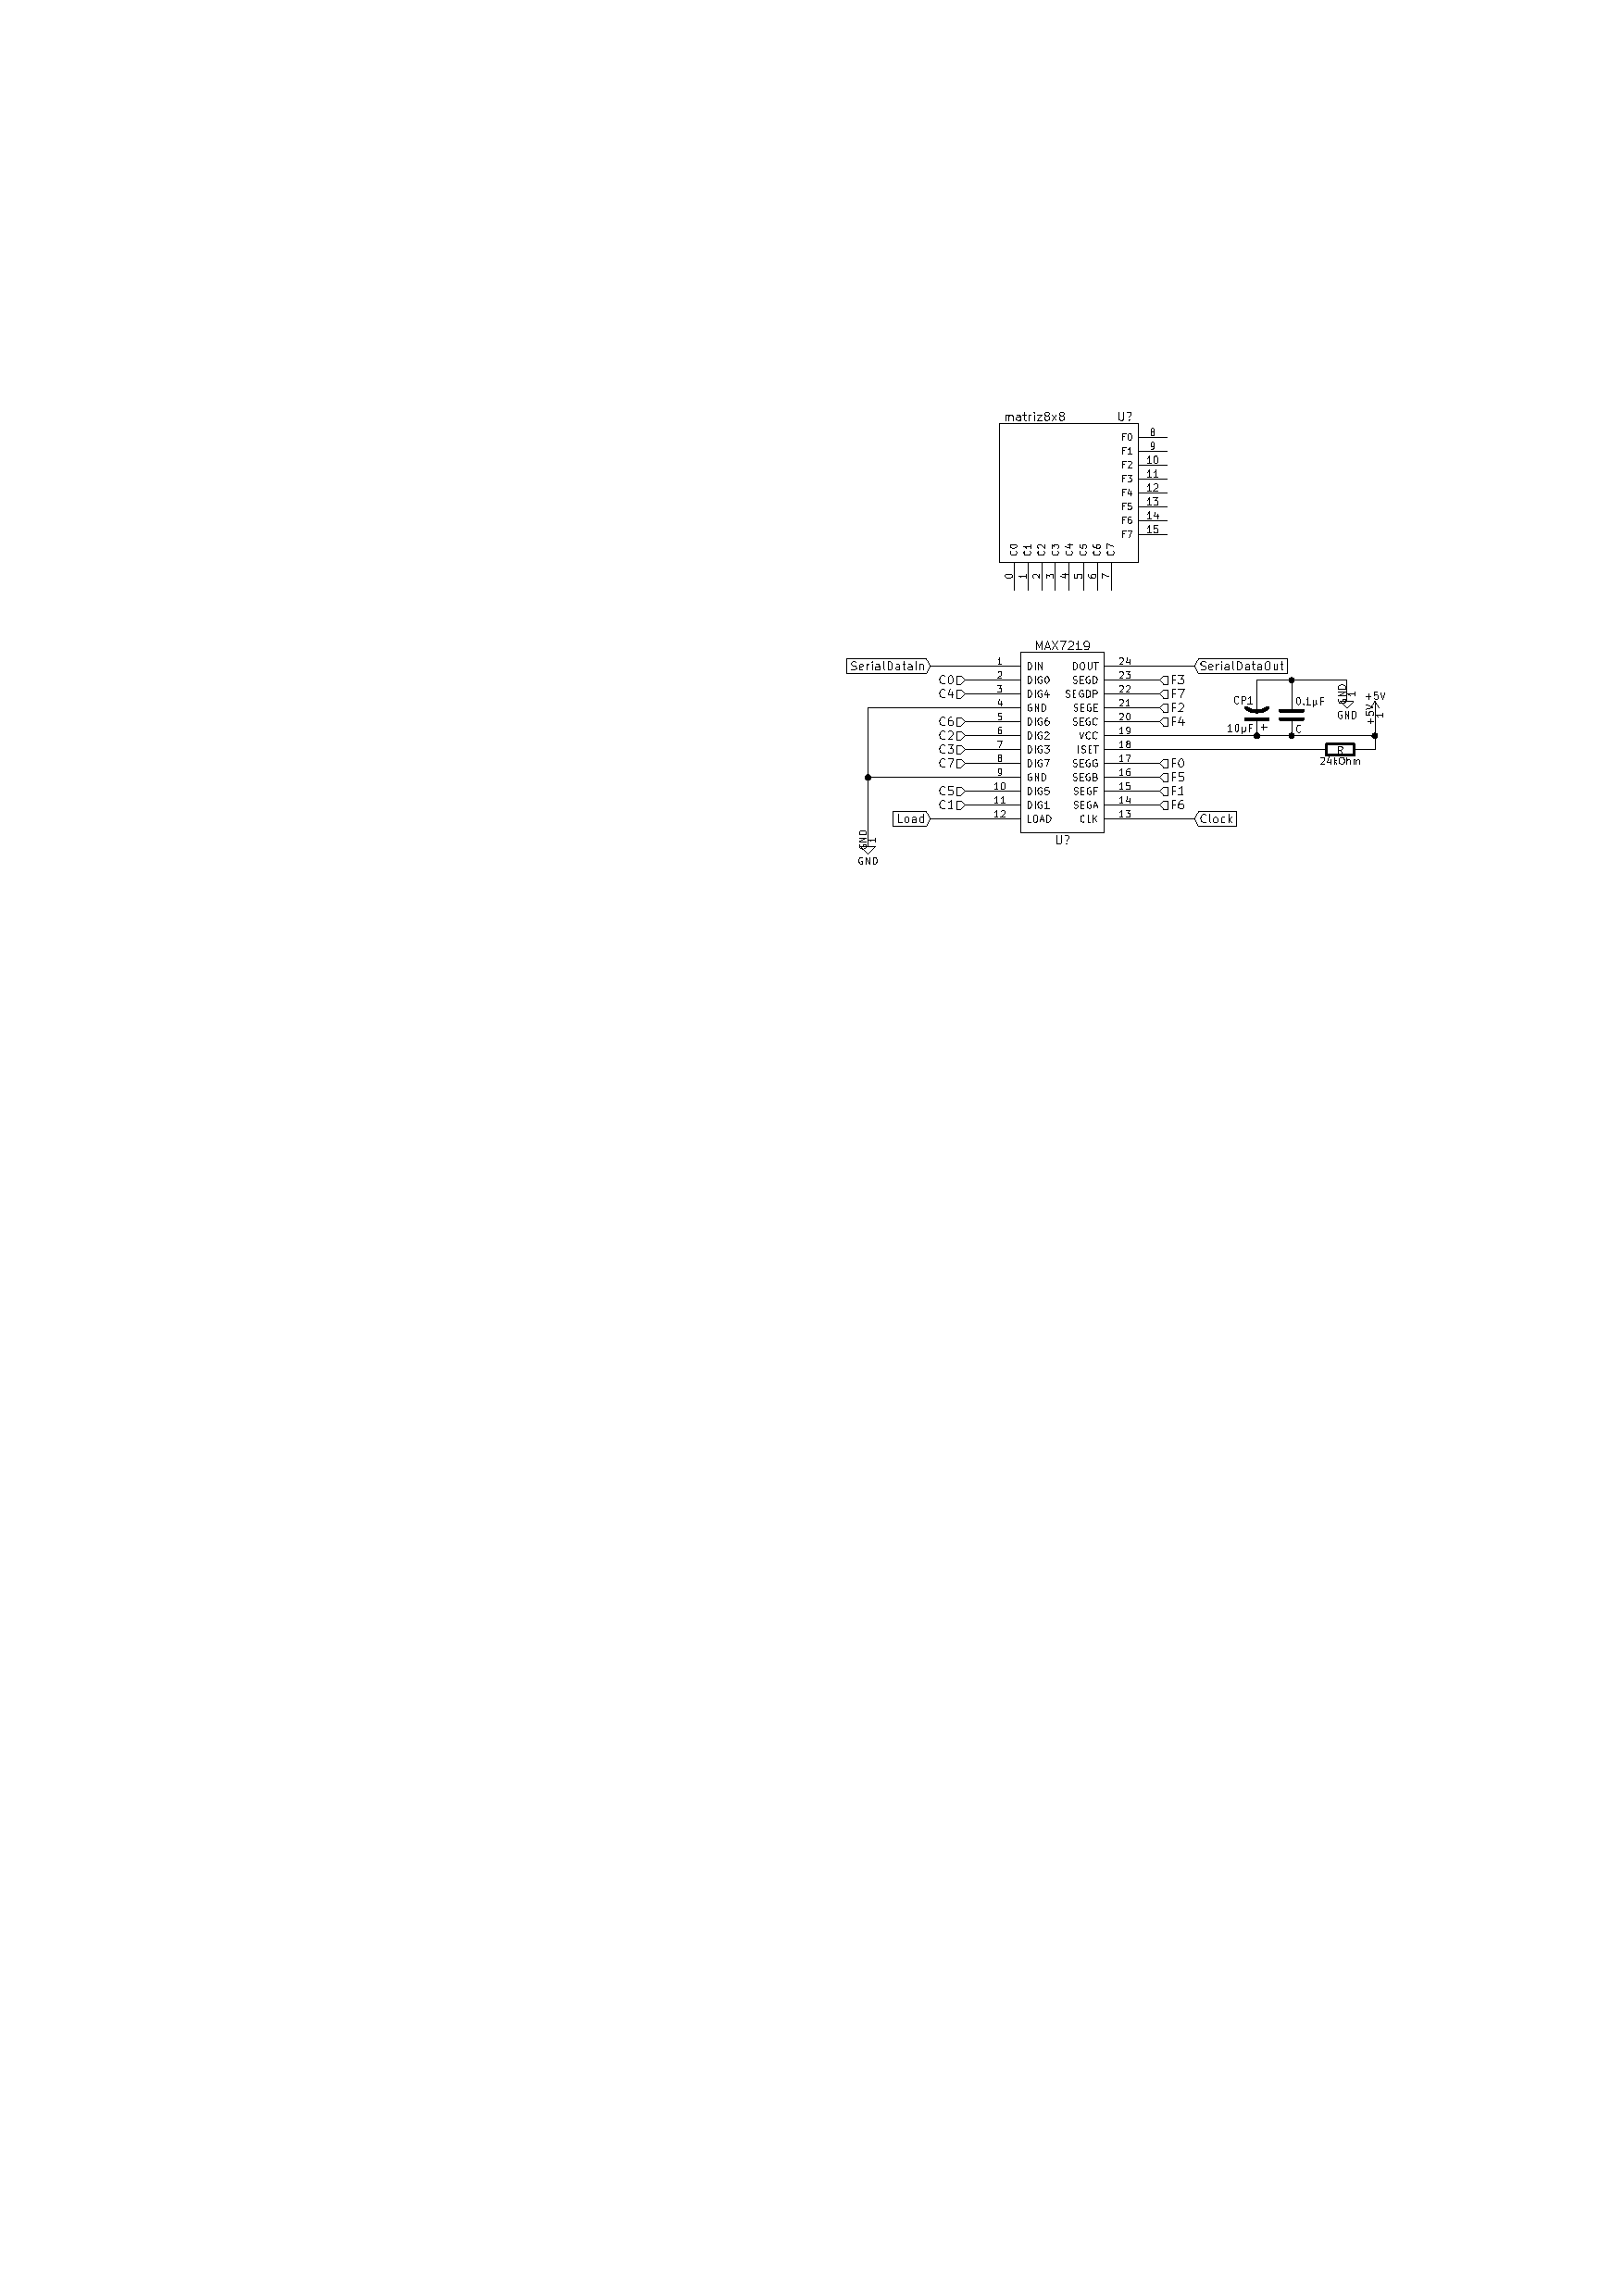
\includegraphics[width=0.8\textwidth]{imagenes/hw/conexion-MAX-matriz.pdf}
	\caption{Conexión entre MAX7219 y su módulo de LEDs.}
	\label{fig:MAX-matriz}
\end{center}
\end{figure}

\begin{figure}[ht!]
\centering
\begin{center}
	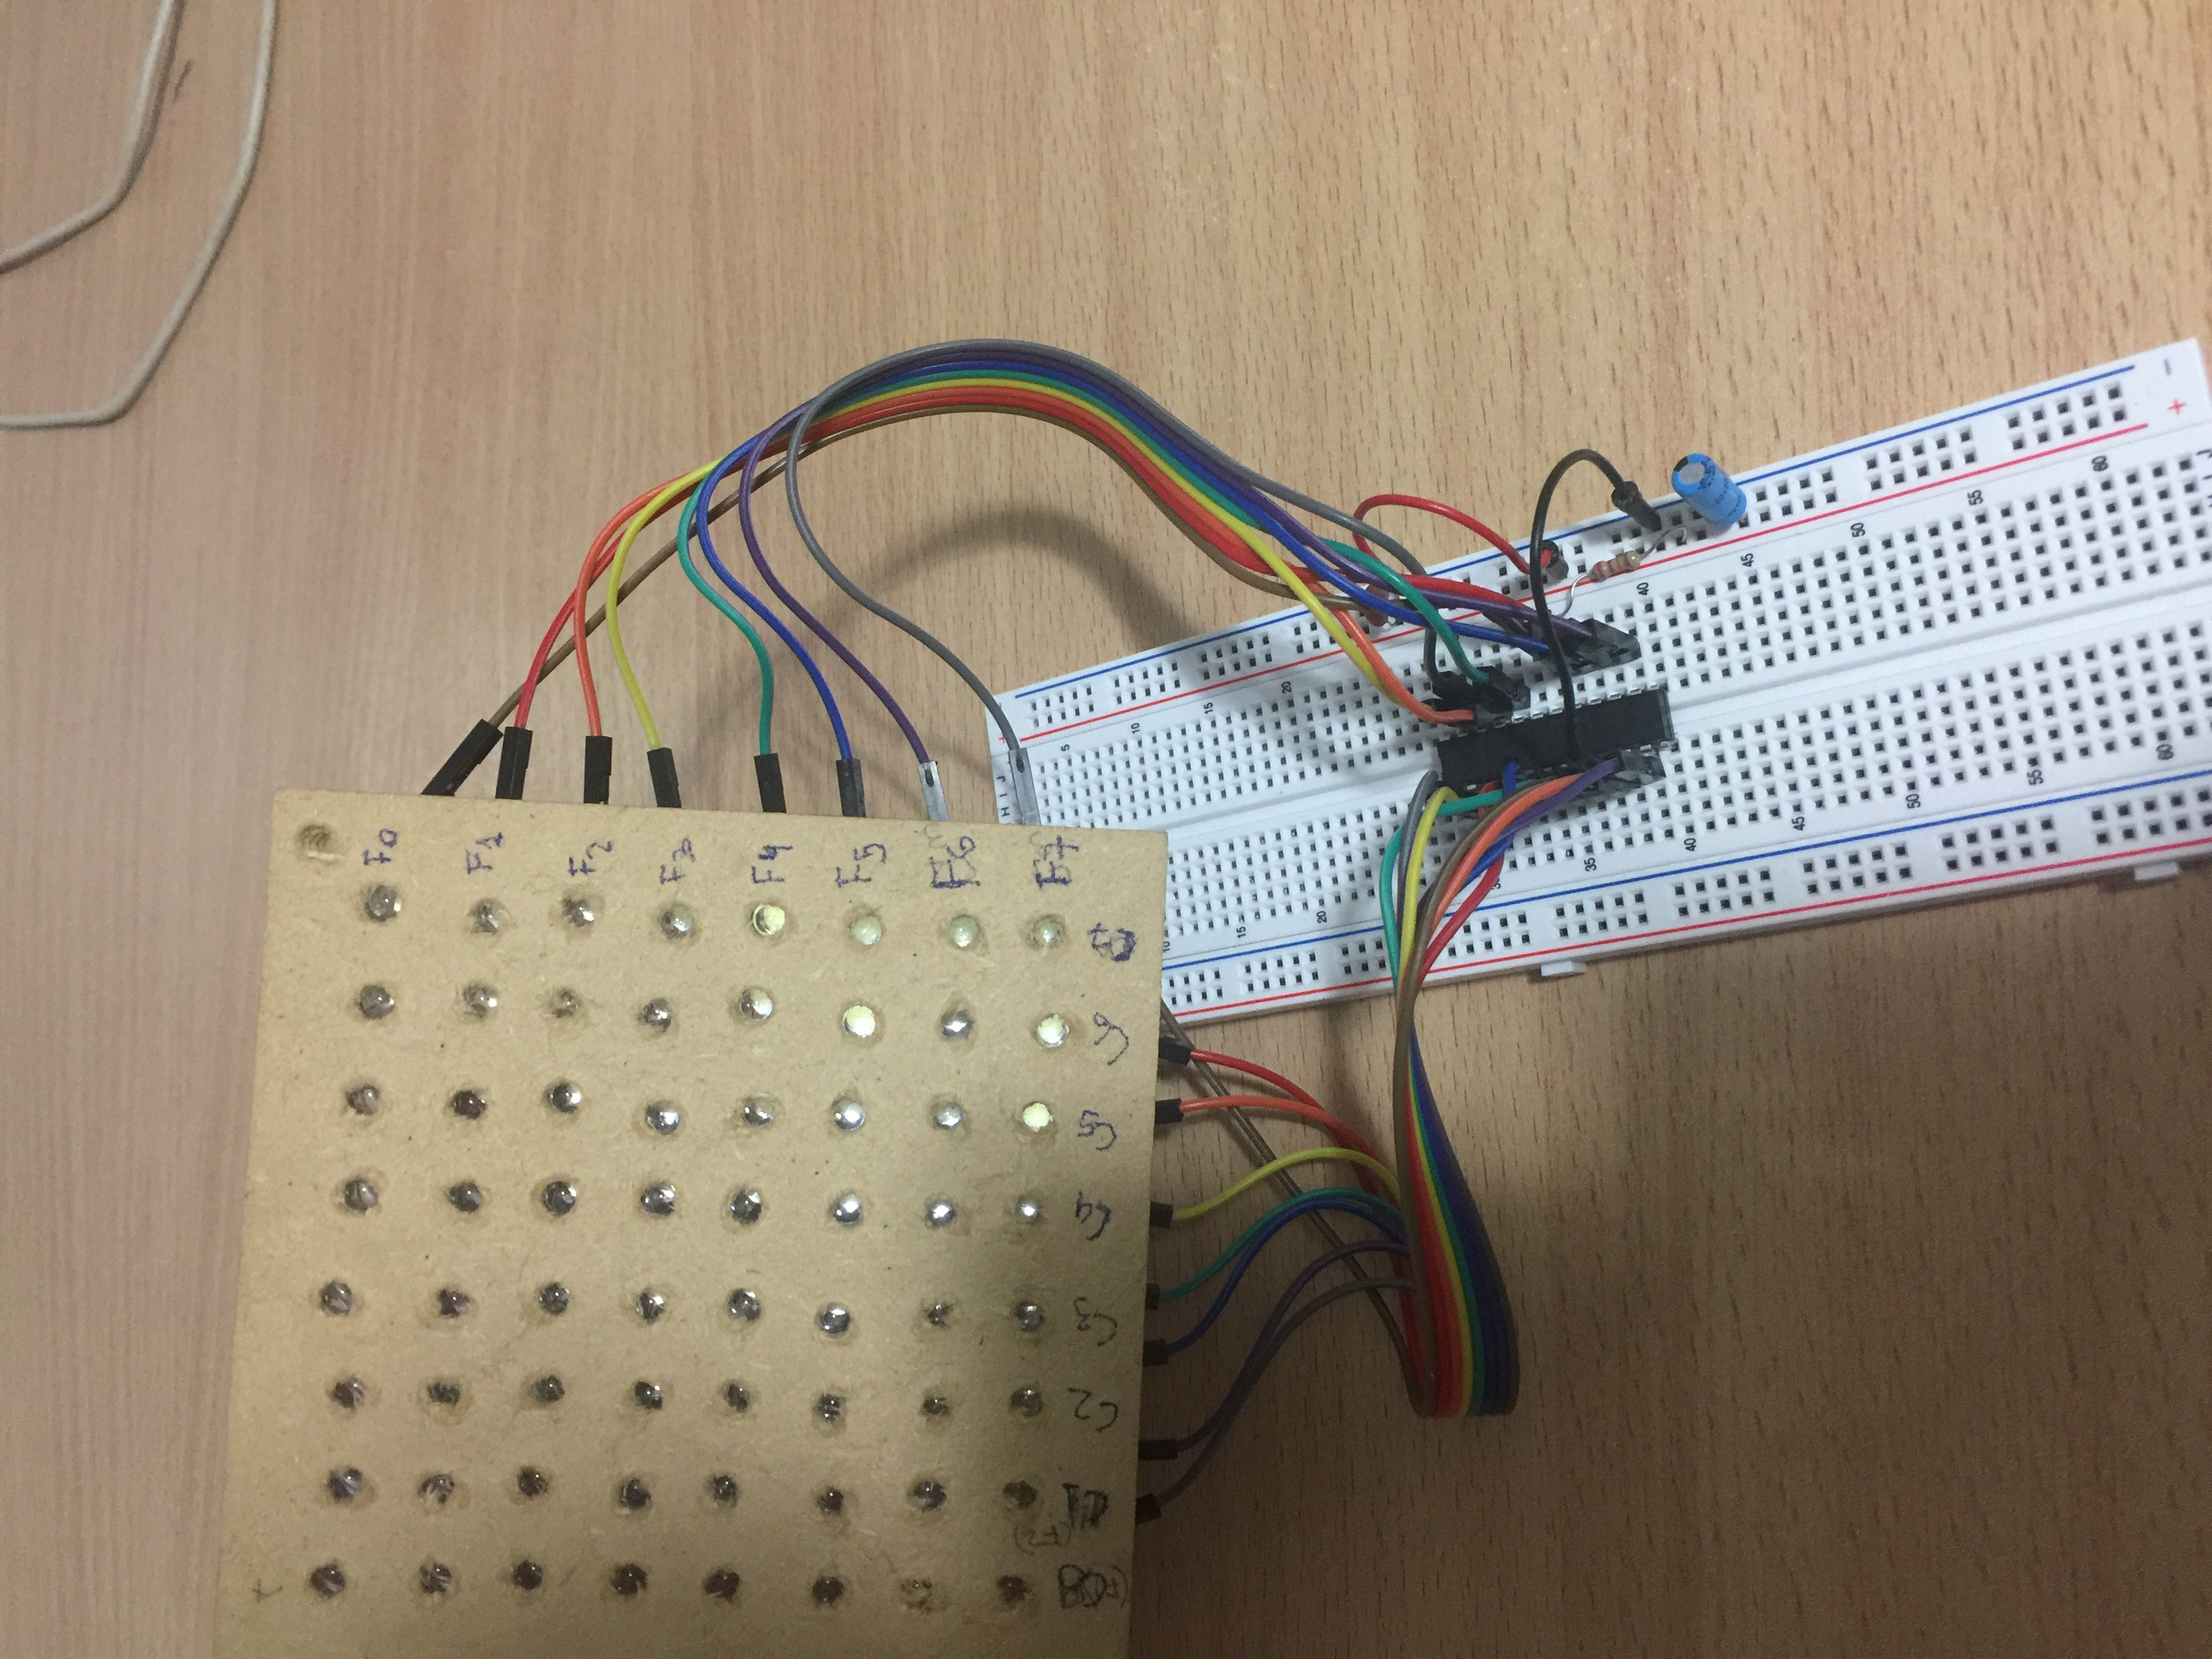
\includegraphics[width=0.7\textwidth]{imagenes/hw/conexion-MAX-matriz.JPG}
	\caption{Fotografía de conexión entre MAX7219 y su módulo de LEDs.}
	\label{fig:MAX-matriz-real}
\end{center}
\end{figure}


\subsection{Matriz de LEDs}
La matriz posee 64 LEDs organizados en ocho filas y ocho columnas, con cátodo común en las columnas como se observa en la figura \ref{fig:modulo-led}. Se analizaron las dimensiones más apropiadas para la utilidad del cartel y se llegó a una separación de 12mm entre LEDs la cual mantiene un dpi apropiado (consiguiendo verse las letras a 10 metros), las demás medidas de pueden observar en la figura \ref{fig:modulo-led-dimensiones}.

Cada uno de los MAX7219 está conectado a una matriz, sus conexiones se pueden observar en el diagrama \ref{fig:MAX-matriz}. Adicionalmente, en la figura \ref{fig:MAX-matriz-real} se observa el prototipo que complementa el esquema de conexión de la figura previamente mencionada.


A la hora de efectuar las conexiones, se debe prestar principal atención a la orientación de la matriz. En la figura \ref{fig:MAX-matriz-real} se indica claramente cuáles son las filas (y su orden) y cuáles son las columnas. Con dicha información el proceso de conexionado se simplifica.

\begin{figure}[!ht]
	\centering
	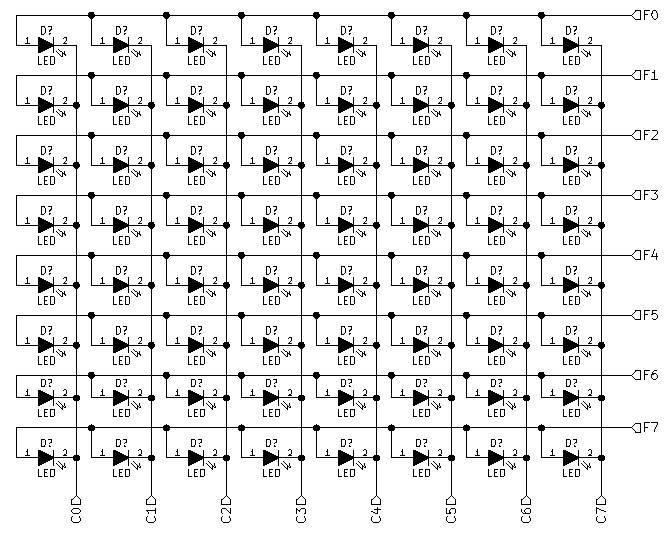
\includegraphics[width=0.7\linewidth]{imagenes/hw/modulo-led.pdf}
	\caption{Esquema de conexiones de la matriz de LEDs.}
	\label{fig:modulo-led}
\end{figure}
\begin{figure}[!ht]
	\centering
	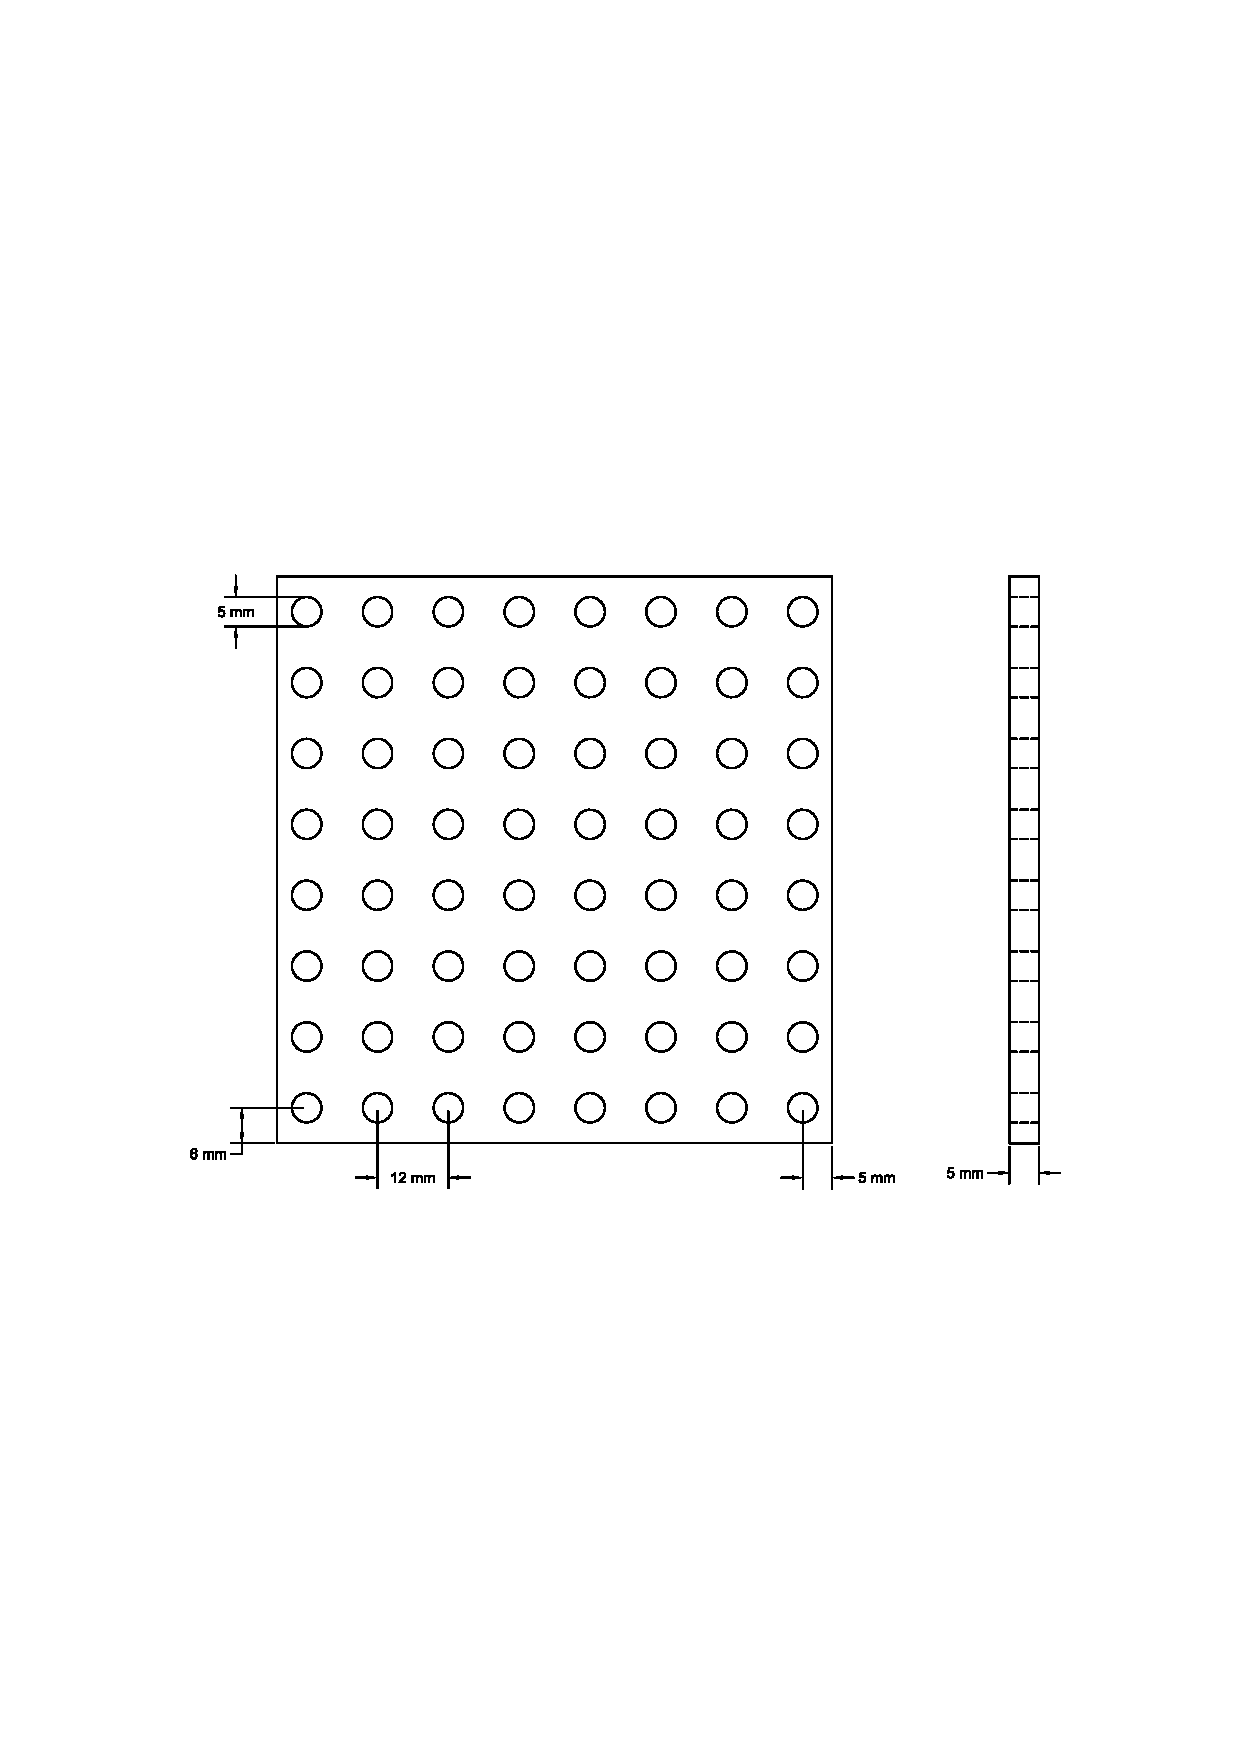
\includegraphics[width=\linewidth]{imagenes/hw/modulo-led-dimensiones.pdf}
	\caption{Dimensiones de la matriz de LEDs.}
	\label{fig:modulo-led-dimensiones}
\end{figure}


\subsection{Comunicación entre los módulos}

\subsubsection{Entre maestro y esclavo}
Como el microcontrolador entrega los datos a 3.3V es necesario convertir estas señales a un voltage que el MAX7219 acepte, la solución que se optó fue incorporar transistores que capaces de transformar 3.3V a 5V. Para ello se conecta tres transistores NPN al circuito, uno por cada señal (DATAIN, LOAD, CLK), se puede observar en la figura \ref{fig:transistors} la conexión.

Los transistores utilizados en el prototipo final son los 2n2369 %(http://www.pci-card.com/2n2369.pdf)
.La base es el pin 2, el colector el pin 1 y el emisor el pin 3.
\begin{figure}[ht!]
	\centering
	\begin{center}
		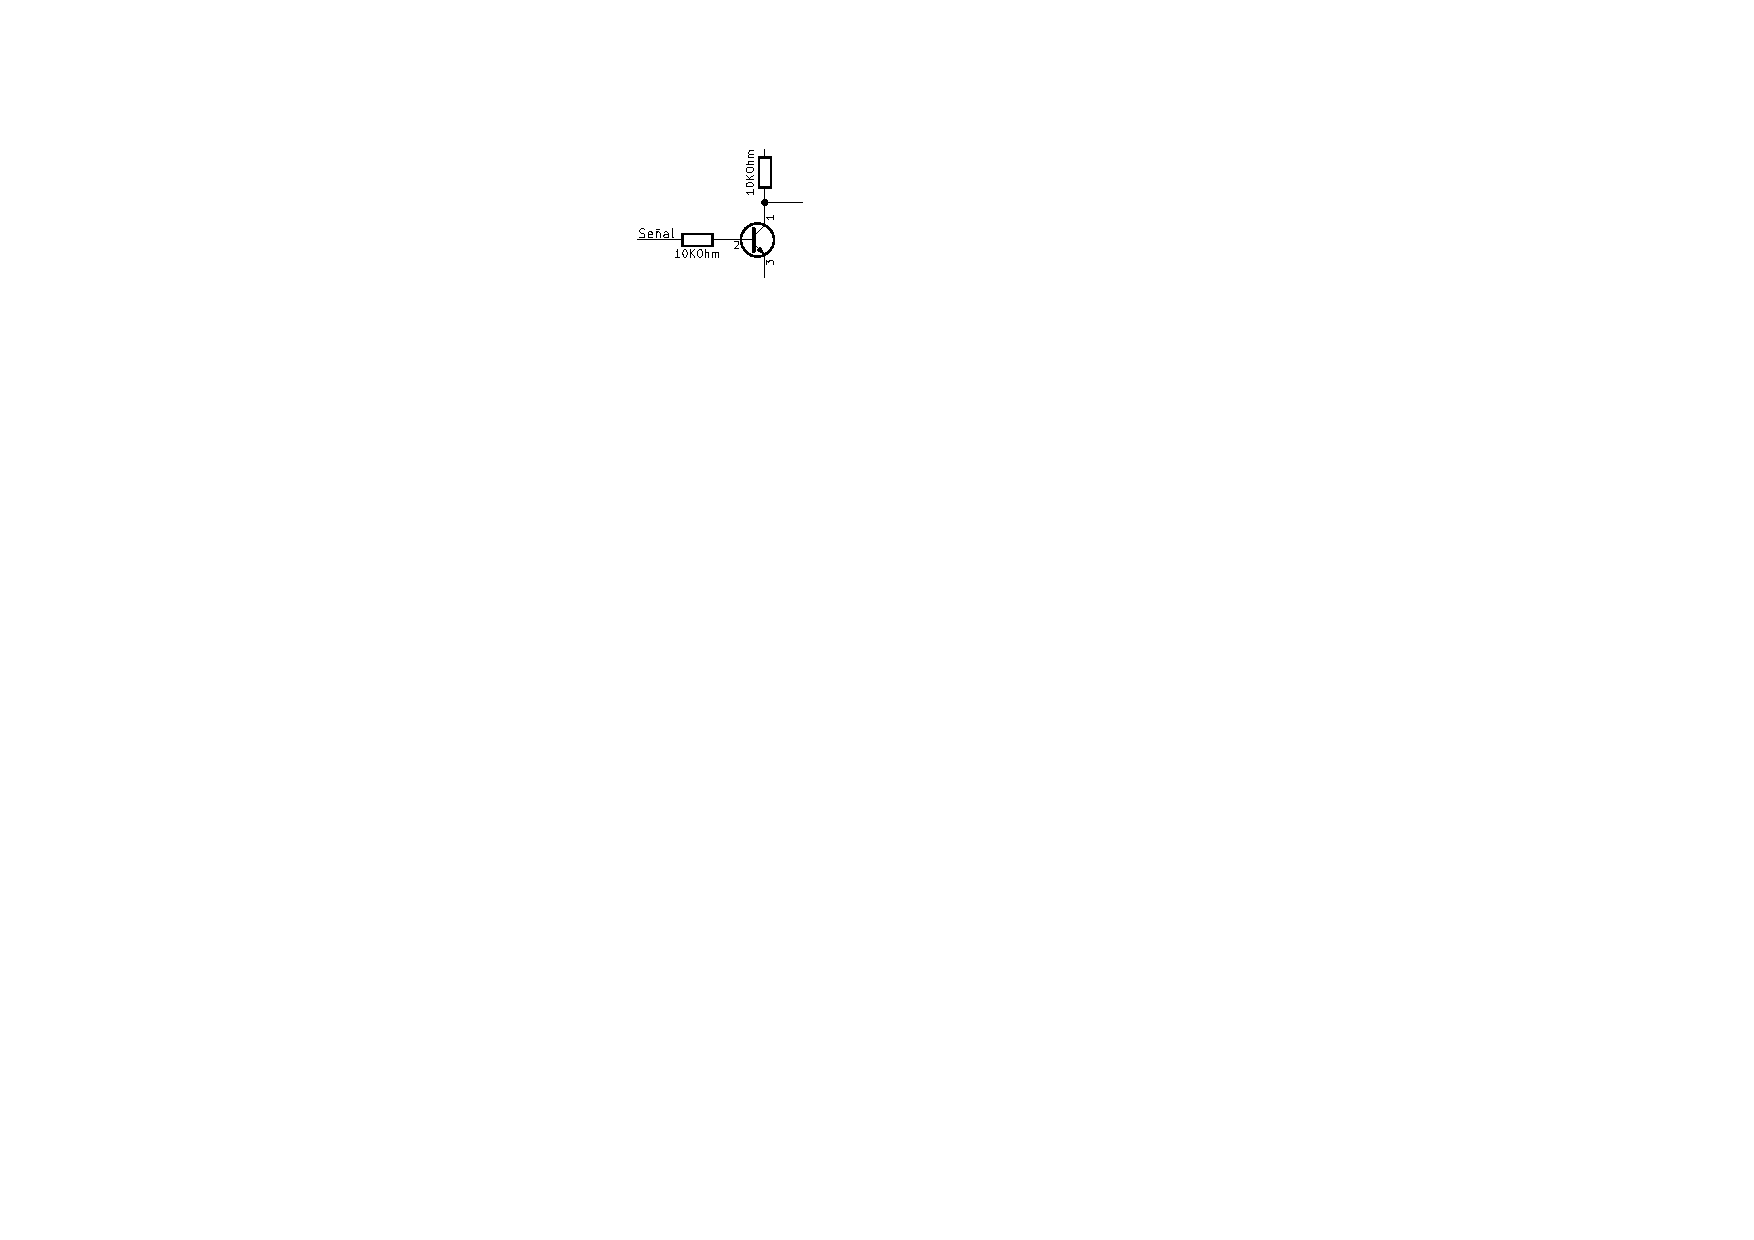
\includegraphics[width=0.7\textwidth]{imagenes/hw/transistor.pdf}
		\caption{Conexión de un transistor, junto con los valores de las resistencias.}
		\label{fig:transistors}
	\end{center}
\end{figure}

\subsubsection{Protocolo de comunicación SPI entre los MAX7219} \label{sec:comunicacion}
Es posible expandir el cartel con N esclavos. En la figura \ref{fig:MAX-MAX} se observa la forma en que se debe realizar la interconexión de los dispositivos integrados.

\begin{figure}[ht!]
	\centering
	\begin{center}
		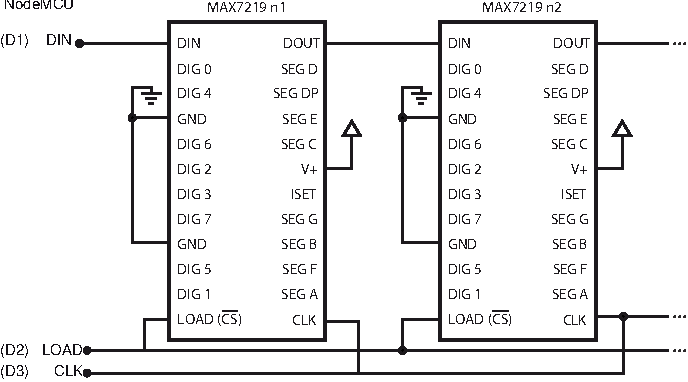
\includegraphics[width=\textwidth]{imagenes/hw/MAX-daisychain.pdf}
		\caption{Conexión entre dos MAX7219.}
		\label{fig:MAX-MAX}
	\end{center}
\end{figure}
Es importante destacar la forma en la que se comunican el microcontrolador con el primer chip shifter, y a su vez, el protocolo que utilizan para comunicarse entre los distintos MAX7219.

La idea general consiste en indicarle a cada chip shifter los leds que debe encender y apagar en cada columna. Para ello debe enviar palabras de dos bytes de manera serial. Es decir, primero envía la información de la columna 1, después la 2, y así siguiendo hasta la 8. El protocolo utilizado es SPI y corresponde a la trama previamente detallada (ver figura \ref{table:trama-spi}).

\begin{table}[ht]
	\centering
	\caption{Trama SPI y su significado.}
	\label{table:trama-spi}
	\begin{adjustbox}{max width=\textwidth}
	\begin{tabular}{|c|c|c|c|c|c|c|c|c|c|c|c|c|c|c|c|}
	\hline
	D15 & D14 & D13 & D12 & D11   & D10   & D9   & D8   & D7 & D6 & D5 & D4 & D3 & D2 & D1 & D0 \\ \hline
	X   & X   & X   & X   & \multicolumn{4}{c|}{ADDRESS} & \multicolumn{1}{c}{ MSB } & \multicolumn{6}{c}{ DATA } & \multicolumn{1}{c|}{ LSB } \\ \hline
	\end{tabular}
	\end{adjustbox}
\end{table}

Para realizar este proceso, la figura \ref{fig:spi-timing-diagram} muestra un diagrama a lo largo del tiempo de la forma de enviar cada bit. En ella se puede observar que el primer paso consiste en bajar la señal de LOAD y esperar un instánte de tiempo (aproximadamente un microsegundo). Luego se debe generar una señal de CLCK de onda cuadrada y de frecuencia de 1Mhz con la mitad de ciclo de trabajo.

El pin conectado al DATAIN del micro, se utiliza para enviar los datos, empezando por el bit más significativo primero. Los datos van a ser leídos por los MAX7219 en el flanco ascendente del CLOCK. Cuando finaliza el envío de los 16 bits, se debe subir la señal de LOAD. En ese momento, el MAX2719 almacena, en sus registros internos, el comando recibido. Todos los comandos son de dos bytes, sin embargo, se puede enviar más de esa cantidad. Esta funcionalidad se utiliza para enviar instrucciones a los demás MAX7219 que están conectados en serie. Lo que ocurre es que la información se recibe en el flanco ascendente de CLK y se envía, hacia el siguiente chip, por el pin DATAOUT en el flanco descendente. De esta forma, en una iteración se pueden configurar una columna de cada módulo de 8x8 LEDs.

\begin{figure}[ht!]
	\centering
	\begin{center}
		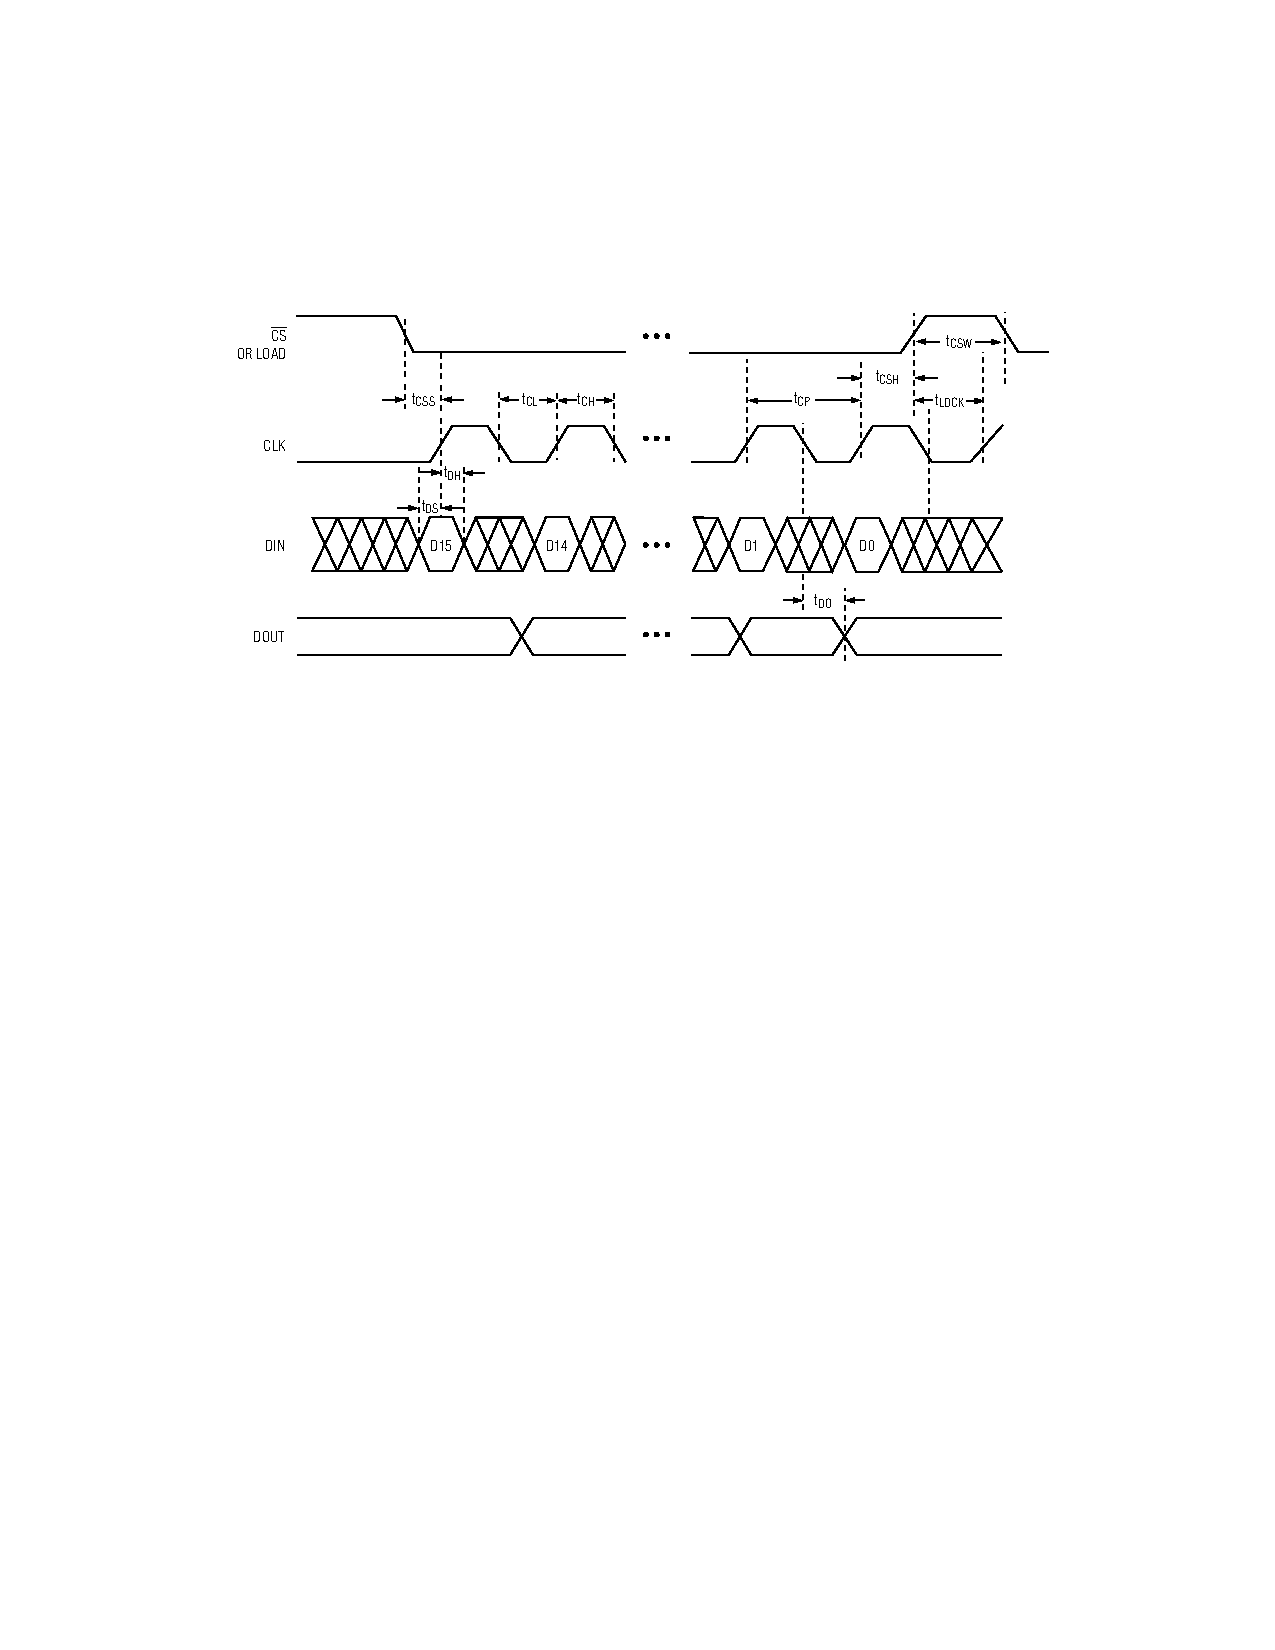
\includegraphics[width=\textwidth]{imagenes/hw/timingDiagram.pdf}
		\caption{Diagrama de tiempo de las señales del MAX7219.}
		\label{fig:spi-timing-diagram}
	\end{center}
\end{figure}


% ==============================================================
\section{Software}\label{sec:sw}
El software del sistema está formado por dos componentes: el firmware que corre sobre el controlador del cartel y la aplicación de PC que corre en una PC.

El cartel ser alcanzable por la PC a través de una red IP. Esto significa que no es estrictamente necesario que la PC y el cartel estén en una misma red física, sino que basta con que exista una ruta entre ellos. Sin embargo, el cartel está asociado a la red estrictamente mediante 802.11 (WiFi), mientras que la PC puede tener conectividad al cartel mediante diversas formas. Detalles básicos sobre el Internet Protocol y mecanismos de routeo no se discutirán en este informe.

\subsection{Interacción PC-Cartel}
La comunicación que se da entre la PC y el cartel sigue el modelo de Cliente-Servidor donde la PC es el cliente y el cartel es el servidor. Esto significa que es la PC quien comienza a interactuar con el cartel, estableciéndose un circuito virtual que permanecera activo cada vez que se quiera hacer un cambio de mensaje o configuración en el cartel, o incluso cuando se quiera recuperar el mensaje del cartel.

El tiempo que permanece activa la conexión debe ser, en lo posible, lo más corto posible. El cartel debe cerrar una conexión que permanezca ociosa por más de un tiempo configurable. La razón de esto es que un individuo malintencionado puede iniciar una conexión hacia el cartel y no mandar ningún mensaje, efectivamente bloqueando el uso legítimo del cartel (por limitaciones técnicas que se explicarán mas adelante, el controlador del cartel sólo puede aceptar una conexión a la vez). Se debe elegir un tiempo (a partir de ahora, tiempo de timeout) lo suficientemente corto para que esta medida sea efectiva pero no tan corto que descarte conexiones que legítimamente tienen un retardo (por ejemplo, por congestión de la red). Este tiempo es una constante ajustable en el código del firmware del cartel.

La figura \ref{fig:petri-net} describe el mecanismo de interacción entre la PC y el cartel mediante una red de Petri.

\begin{figure}[htbp]
	\centering
	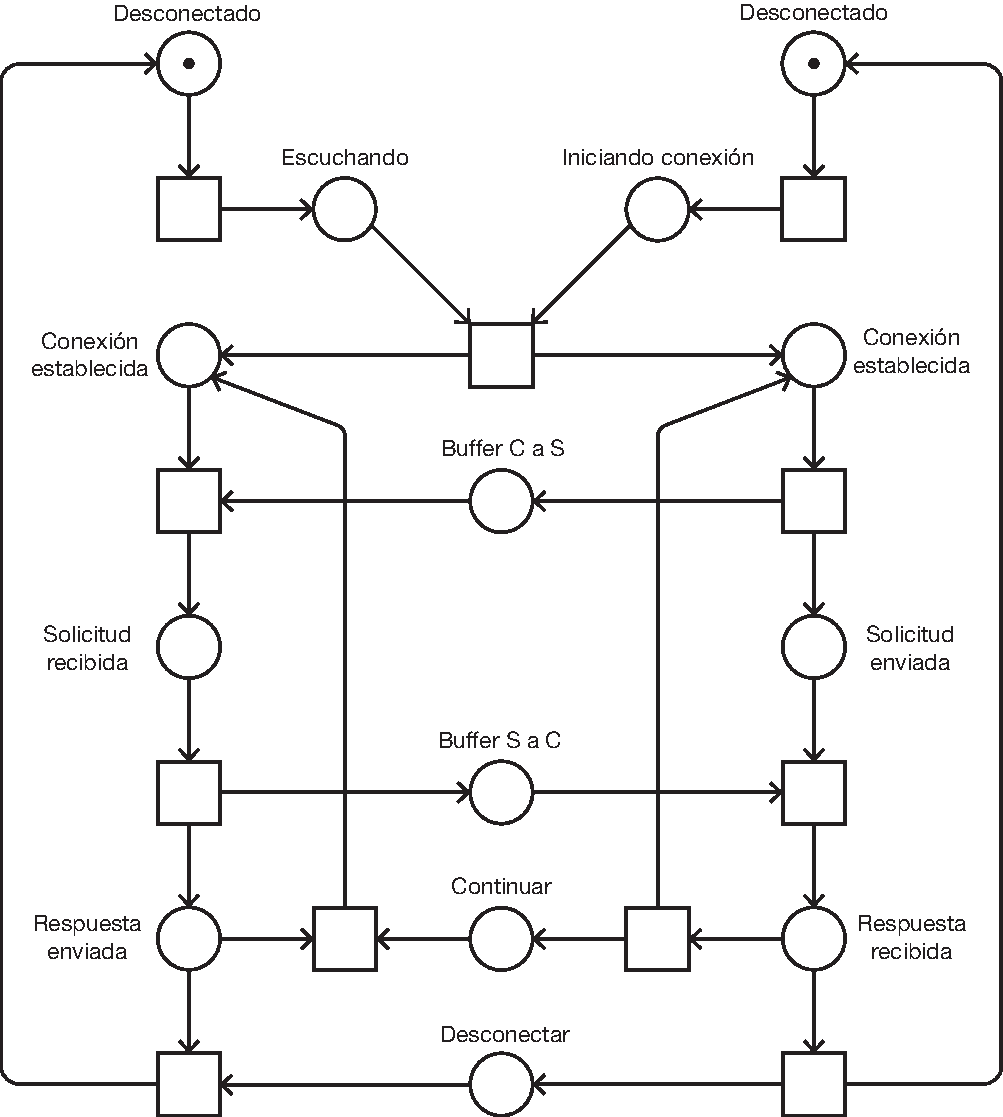
\includegraphics[width=\linewidth]{imagenes/petri-net.pdf}
	\caption{Red de Petri modelando la interacción entre la aplicación de PC y el cartel.}
	\label{fig:petri-net}
\end{figure}

\subsection{Firmware}
El firmware del controlador del cartel es quien se encarga de aceptar pedidos de la aplicación de PC y ejecutar las acciones de cambio de mensaje, parámetros de animacion, configuración WiFi o de contraseña. Además, como se explicó en la sección \ref{sec:hw}, el ESP8266EX envía la configuración de las matrices de LED por serie.

\subsection{Plataformas de desarrollo}
El System on Chip ESP8266EX es muy popular y existen diversas formas de desarrollar para él, entre ellas están:
\begin{itemize}
	\item El SDK oficial \enquote{OS} de Espressif. Es un SDK privativo. Utiliza internamente FreeRTOS con lo que se puede programar con tareas y las primitivas de sincronización que FreeRTOS ofrece.
	\item El SDK oficial \enquote{NON-OS} de Espressif. Tiene \enquote{NON-OS} en su nombre porque con este SDK el programador no puede especificar ni crear tareas propias. Sino que se limita a registrar funciones callbacks que son llamadas por el firmware de Espressif cuando suceden eventos. La programación termina siendo basada en eventos.
	\item La implementación de la plataforma Arduino para el ESP8266EX. Es la más sencilla de utilizar. Tiene las mismas abstracciones que se utilizan en la plataforma Arduino original. Incluye clases C++ que implementan servidores HTTP y hay mucho software y soporte disponible.
\end{itemize}

Todas estas formas de desarrollar tienen en común que el software del programador corre sobre un firmware privativo, es decir, no es viable programarlo \enquote{bare-metal} porque los registros y todos la información del hardware necesario para realizar algo no trivial no está disponible.

Para el este proyecto se decidió utilizar el SDK \enquote{NON-OS}, donde las funciones que define el programador se ejecutan siempre enteramente, de forma cooperativa. Esto elimina toda una clase de problemas de interferencia de datos a causa de la concurrencia, con lo que no es necesario utilizar primitivas de sincronización.
\subsubsection{Arquitectura del software}
\subsection{Aplicación de PC}
La aplicación de PC es un programa con interfaz gráfica que permite al usuario administrar el contenido y configuración del cartel de forma remota. En el marco del protocolo definido en el \ref{sec:protocolo}, la aplicación de PC es el cliente.

\subsubsection{Plataforma de desarrollo}
La aplicación está desarrollada en el \emph{framework} de desarrollo Qt. Qt es un conjunto muy amplio de librerías que permiten el desarrollo de aplicaciones gráficas que se pueden compilar para distintas plataformas (Windows, GNU/Linux, macOS o cualquier variante de Unix con X11). El lenguaje de programación que se utiliza es C++ con extensiones propias de Qt.

\subsubsection{Arquitectura basada en eventos}\label{sec:qt}
Qt permite desarrollar aplicaciones con una arquitectura basada en eventos. Sin embargo, la implementación de este sistema de eventos no está basada en los mecanismos más clásicos como el patrón Observer de la programación orientada a objetos ni el mecanismo de callbacks o punteros a funciones propios de la programación procedural, sino que hay métodos en los objetos que pueden ser denominados \emph{signals} o \emph{slots}.

Una clase puede tener opcionalmente uno o más métodos que sean \emph{signal} o \emph{slot}. La idea clave de estas sistema es que un objeto puede \enquote{emitir} una \emph{signal} que ejecuta el método \emph{slot} de otro objeto (o incluso posiblemente el mismo emisor) al cual se estableció previamente lo que se denomina \enquote{conexión}. Se ilustra este mecanismo en la figura \ref{fig:signals-slots}

\begin{figure}[!ht]
	\centering
	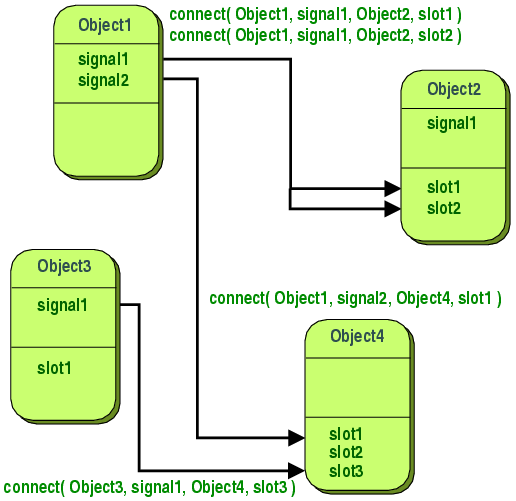
\includegraphics[height=8cm]{imagenes/signal-slots.png}
	\caption{Mecanismo de \emph{signal} y \emph{slot}.}
	\label{fig:signals-slots}
\end{figure}

En Qt, las clases que necesiten utilizar el sistema de eventos deben heredar de una clase provista por la librería llamada \code{QObject}. Esta clase provee distintas funcionalidades al resto de las clases definidas por Qt. Entre los objetos que heredan de QObject puede existir una relación de parentesco, en la cual un objeto $B$ puede tener como padre a otro objeto $A$. Esto, por ejemplo, sirve para liberar al programador del manejo de memoria: un objeto puede destruir a sus hijos antes de destruirse a sí mismo (por destrucción se entiende la liberación de todo recurso asociado al objeto, como memoria o archivos).

El mecanismo de \emph{signal} y \emph{slots} tiene como una de sus ventajas el hecho de que la ejecución de un \emph{slot} darse en otro hilo. Esto esta relacionado con la idea que promueve Qt de que un objeto puede "pertenecer" a un hilo de ejecución (encapsulado por la clase \code{QThread}), esto permite que no haya interferencia de datos causada por la concurrencia ya que no hay accesos explícitos a variables compartidas entre hilos sino que pueden enviar datos como argumentos a los \emph{slots}, de forma similar al paradigma de pasaje de mensajes en programación concurrentes.

Por ejemplo, en el caso del objeto \code{Object1} en la figura \ref{fig:signals-slots}, en algún método suyo se podría tener código como el siguiente:
\begin{lstlisting}[language=c++]
	// ...
	emit signal1();
	// ...
\end{lstlisting}

Mientras que \code{Object2} tiene un \emph{slot} llamado \code{slot1()} al cual \code{signal1()} de \code{Object1} está conectado. Entonces al emitirse \code{signal1()}, se ejecuta también \code{slot1} de \code{Object2} (además de los otros métodos pertenecientes a las otras clases que aparecen en la figura).

El momento en que se ejecuta un \emph{slot} depende del tipo de conexión que se haya establecido entre los objetos. Qt define tres tipos de conexiones:
\begin{description}
	\item[\code{DirectConnection}:] el \emph{slot} se ejecuta en el mismo hilo de ejecución desde el cual se hizo la emisión. Esto es útil para cuando los objetos que están conectados pertenecen a un mismo hilo o también cuando pertenecen a distintos hilos pero se toma precaución utilizando primitivas de sincronización para serializar el acceso al recurso o memoria compartida.
	\item[\code{QueuedConnection}:] se coloca un pedido de ejecución de \emph{slot} (con los argumentos que se hayan emitido) en la cola de eventos del hilo del objeto destino. Esto es lo que libera al programador de tener que utilizar primitivas de sincronización explícitas y es lo que se usa mayormente en la aplicación de PC de este proyecto. La ejecución de \code{emit} retorna inmediatamente, con lo que el hilo del objeto emisor no se bloquea al emitir una señal.
	\item[\code{BlockingQueuedConnection}:] Similar a \code{QueuedConnection}, con la diferencia que el hilo emisor se bloquea hasta que finalice la ejecución de los \emph{slots} que haya activado. Si no se utiliza con precaución y se establecen conexiones cíclicas, existe el riesgo de que ocurra un \emph{deadlock}, ocurrencia en la que un conjunto de hilos se espera entre sí indefinidamente, deteniendo parcial o íntegramente el programa.
\end{description}

Internamente, la implementación de Qt tiene una cola bloqueante de eventos para cada uno de los hilos que tengan una instancia de la clase \code{QThread}. También lleva registro de cuáles objetos que heredan de \code{QObject} pertenecen a cuál hilo. De esta manera, la ejecución de un hilo consiste principalmente en esperar a que hayan eventos para procesar en una cola bloqueante, cuya implementación específica depende de la plataforma para la cual se esté compilando el programa.

\subsubsection{Módulos}
En esta sección se listan las clases más relevantes de la aplicación de PC, sus métodos públicos principales y la interacción entre ellos.
Las clases son:
\begin{description}
	\item[\code{Panel}:] Provee la interfaz gráfica principal, que consiste en una ventana con los distintos elementos de control para que el usuario pueda manipular el cartel. Se puede ver una captura de pantalla en la figura \ref{fig:panel-screenshot}.
	\item[\code{Client}:] Realiza la interacción con el cartel a nivel mensaje del protocolo. Se encarga de generar los mensajes salientes y de tomar las acciones pertinentes ante una respuesta del cartel (servidor). La (única) instancia de esta clase \enquote{pertenece} (ver sección \ref{sec:qt}) a otro hilo en el cual se realizan todas las operaciones bloqueantes de entrada y salida, de forma que no se bloquea el hilo principal, que causaría que la interfaz gráfica deje de responder a eventos del sistema o del usuario.
	\item[\code{Connection}:] Abstrae la conexión al cartel, exponiendo métodos que envían y reciben específicamente los mensajes definidos en el protocolo. En esta clase también se hace la carga del certificado TLS antes de establecer una conexión.
	\item[\code{SignModel}:] Una clase \enquote{tonta} que agrupa todos los parámetros modificables del cartel, como el texto del cartel y sus parámetros de animación, los datos de la red Wifi a la que se debe conectar el cartel, etc. Existe principalmente para llevar registro de cuales parámetros fueron cambiados por el usuario y ameritan un pedido de cambio hacia el cartel. De manera que no se hagan cambios innecesarios al contenido o configuración del cartel.
\end{description}

\begin{figure}[!ht]
	\centering
	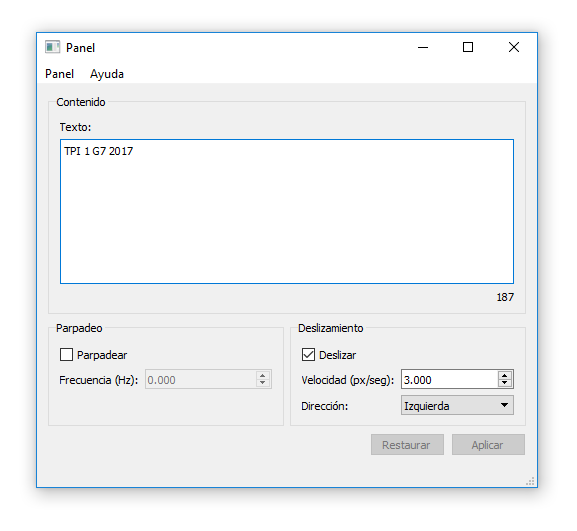
\includegraphics[height=10cm]{imagenes/panel-screenshot.png}
	\caption{captura de pantalla de la ventana principal de la aplicación de pc.}
	\label{fig:panel-screenshot}
\end{figure}

Se puede ver en la figura \ref{fig:uml-cliente} un diagrama de los objetos mencionados anteriormente. No están incluidas las conexiones entre los objetos para mantener la prolijidad del diagrama.

\begin{figure}[!ht]
	\centering
	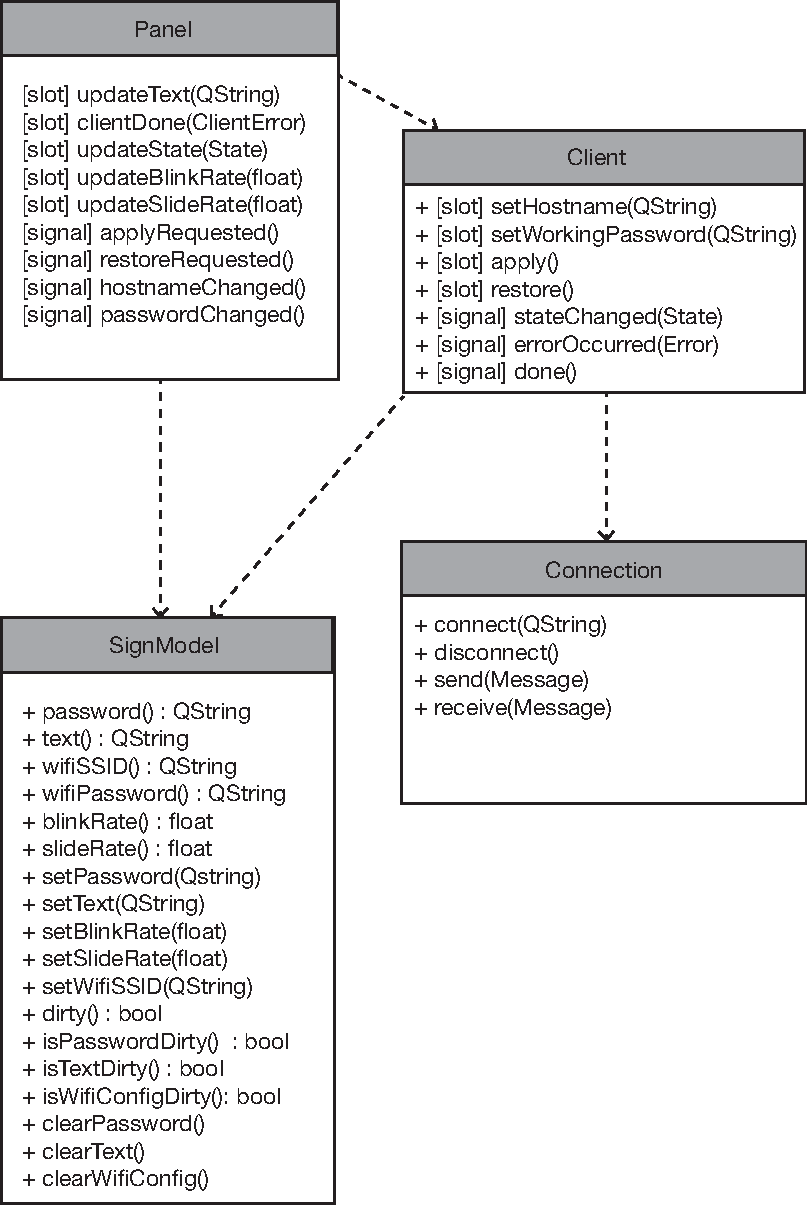
\includegraphics[scale=0.8]{imagenes/uml-cliente.pdf}
	\caption{Diagrama UML de las clases más relevantes.}
	\label{fig:uml-cliente}
\end{figure}

\subsection{Protocolo de comunicación}\label{sec:protocolo}
\subsubsection{Transport Layer Security}\label{sec:tls}


\clearpage
\part{Ensayos y mediciones}\label{part:ensayos}
\section{Conclusiones}

Pudo comprobarse a través de este proyecto la viabilidad tanto en términos de hardware como de software del diseño planteado como implementación del cartel programable de LEDs. 
La totalidad del protocolo de comunicación pudo ser implementada de acuerdo a lo pautado en los objetivos iniciales, y en tiempo y forma respecto al cronograma propuesto. El desarrollo del hardware se vio demorado por falta de disposición de recursos, ya que algunos componentes no se encuentran disponibles en todas las tiendas de electrónica (Node MCU y MAX7219). Aún así pudo implementarse un prototipo del circuito maestro y dos prototipos de los circuitos esclavos, con las debidas interfaces para las conexiones externas e internas, tanto de datos como de alimentación, y cumpliendo los patrones de diseño recomendados por el personal técnico de la Facultad.
En términos de consumo, se comprobó que la potencia consumida por el circuito coincidía con la calculada mediante los datos indicados en la hoja de datos del MAX7219. Dicho consumo es relativamente bajo, por lo que no se lo considera un impedimento relevante a la hora de conseguir nuevas fuentes de alimentación para el sistema. 
Aunque no estaba planificado en el proyecto inicial el equipo también adaptó un cargador móvil en desuso para alimentar el circuito.
((como hacemo lo de las horas?))

El presupuesto del proyecto cumplió con exactitud con lo planteado en la sección homónima del anexo.
% Explicar el grado de cumplimiento de objetivos planteados para el trabajo.
% Evaluar y destacar el cumplimiento y disvíos del cronograma de tareas presentados en el informe inicial
% Describir claramente la actividad de cada integrante del grupo, evaluar las horas invertidas por cada uno y calcular las horas de ingeniería total
% Analizar el presupuesto que se ha invertido y el presupuesto final del proyecto incluyendo las horas de ingeniería consumidas.

	\clearpage
	\printglossary[type=\acronymtype, title=Siglas y acrónimos, toctitle=Siglas y acrónimos]
 	\printglossary[title=Glosario, toctitle=Glosario]

	\phantomsection
	\bibliography{biblio}

	\appendix
\clearpage
\addappheadtotoc
\appendixpage

\setcounter{figure}{0}

\section{Desarrollo de PCB}

\end{document}